\subsection{Monte-Carlo}
\label{ssec:montecarlo}
Esta sección explica el método de Monte-Carlo aplicado a los problemas de búsqueda en árboles de juegos.
Se estudia una versión básica del mismo y se presentan los agentes que lo usan.

El \textbf{método de Monte-Carlo} consiste en realizar un número de simulaciones a partir del estado actual para decidir el próximo movimiento.

Una \textbf{simulación} es una partida al azar completa del juego desde la posición actual; es decir, partiendo del estado actual en el árbol de juegos, se realizan movimientos aleatorios hasta llegar a un estado terminal, donde se asigna el valor de utilidad (+1, -1 ó 0 si es el estado es ganador, perdedor o empate para el jugador).
Este valor es usado como la recompensa esperada que se puede obtener a partir del estado sucesor elegido.
Para estimar el valor final de un estado se toman estadísticas haciendo un promedio de las recompensas obtenidas en las simulaciones.

El método genera una lista de posibles movimientos (sucesores del estado actual) y para cada movimiento realiza miles de simulaciones (partidas al azar), obteniendo el valor de recompensa.
El movimiento con un valor de recompensa mayor es el elegido como mejor movimiento, es decir, aquel que conduce a la mejor serie de partidas al azar para el jugador actual.

La ventaja de esta técnica es que requiere poco conocimiento del entorno, pero se incrementan los requisitos computacionales (procesador y memoria).
Para que el método sea efectivo se deben realizar muchísimas simulaciones, ya que los movimientos de las simulaciones se generan al azar y es posible que una buena jugada sea evaluada erróneamente como una mala jugada.

A priori es difícil establecer de antemano un número determinado de simulaciones, por lo que se suele dejar un tiempo máximo para realizar las simulaciones.

\bigskip
Los siguientes apartados presentan dos agentes que usan el método de Monte-Carlo: uno con un número determinado de simulaciones y otro con un límite de tiempo para realizar las simulaciones.

\subsubsection{Monte-Carlo con número de simulaciones fijas}
\label{sssec:montecarlo_simulaciones}
El jugador Monte-Carlo más simple es aquel que tiene un número de simulaciones determinado.

Partiendo del estado actual juega el número de partidas indicadas para evaluar el mejor movimiento.
Para cada sucesor del estado actual se realiza un número diferente de simulaciones, pues estos también son elegidos aleatoriamente.
El número de simulaciones debe ser suficientemente grande para asegurarse de que se realizan aproximadamente el mismo número de simulaciones para cada posible movimiento.
Si \textit{N} es el número total de simulaciones a realizar y \textit{p} es el número de sucesores del estado actual, se espera que se realicen $p/N$ simulaciones para cada movimiento.
Esto sólo se cumple cuando \textit{N} tiende a infinito.

Asignar de antemano un número determinado de simulaciones es una tarea complicada.
Juegos con un espacio de estados mayor requieren mayor número de simulaciones, pero el tiempo de cómputo necesario también es mucho mayor.

\bigskip
El siguiente agente incorpora un límite de tiempo para realizar las simulaciones.

\subsubsection{Monte-Carlo con límite de tiempo}
\label{sssec:montecarlo_limiteTiempo}
El segundo agente que emplea el método de Monte-Carlo dispone de un límite de tiempo para realizar simulaciones.

Se trata de otro algoritmo \textit{anytime}; devuelve mejores soluciones a medida que aumenta el tiempo disponible para realizar la búsqueda, en este caso para realizar las simulaciones.

Asignar un tiempo límite para Monte-Carlo tampoco es tarea sencilla pues no conocemos el tiempo necesario que necesita cada simulación.
La simulaciones deben completarse totalmente para que sean válidas.
No tiene sentido dejar un sólo segundo para realizar simulaciones si cada simulación dura más de un segundo.
En ese caso el tiempo disponible del agente se extenderá hasta el tiempo necesario para terminar la simulación.

Por simplicidad, al igual que ocurre con la estrategia minimax con tiempo limitado (seccion~\ref{sssec:limite_tiempo}), la unidad de tiempo escogida ha sido el segundo.

\bigskip
Una vez presentado el método básico de Monte-Carlo, se explica una versión mejorada del mismo: Monte-Carlo Tree Searh.
También se describen los agentes que usan esta nueva versión.

\subsection{Monte-Carlo Tree Search}
\label{ssec:monteCarloTreeSearch}
Esta sección detalla la estrategia Monte-Carlo Tree Search, basada en el método tradicional de Monte-Carlo explicado en la sección anterior.
Se describen también los dos agentes desarrollados que usan esta técnica.

\bigskip
\textbf{Monte-Carlo Tree Search} (MCTS a partir de ahora) consiste en realizar un número de simulaciones a partir del estado actual para decidir el próximo movimiento, igual que hace el método básico de Monte-Carlo; pero dispone además de un árbol propio para almacenar la información obtenida en las simulaciones y poder usarla para mejorar las propias simulaciones y por tanto la decisión final.

Para no confundir el árbol de búsqueda de los propios juegos con el árbol de búsqueda que emplea el método MCTS llamaremos a este último: árbol de Monte-Carlo (árbol MC).

Antes de cada simulación, MCTS realiza primero una búsqueda en el árbol de juegos a partir de la posición actual hasta encontrar un nodo que no se encuentre en el árbol MC (inicialmente el árbol MC está vacío).
Para realizar esta búsqueda se utiliza una estrategia o política basada en la información almacenada en el árbol MC.
El nuevo estado encontrado se añade al árbol MC y a partir de esa posición se realiza una simulación completa hasta el final de la partida, obteniendo el valor de utilidad del estado terminal.
Con el valor de utilidad obtenido se actualiza la información de los estados visitados en el árbol MC durante la simulación.
\begin{figure}[h]
	\centering
	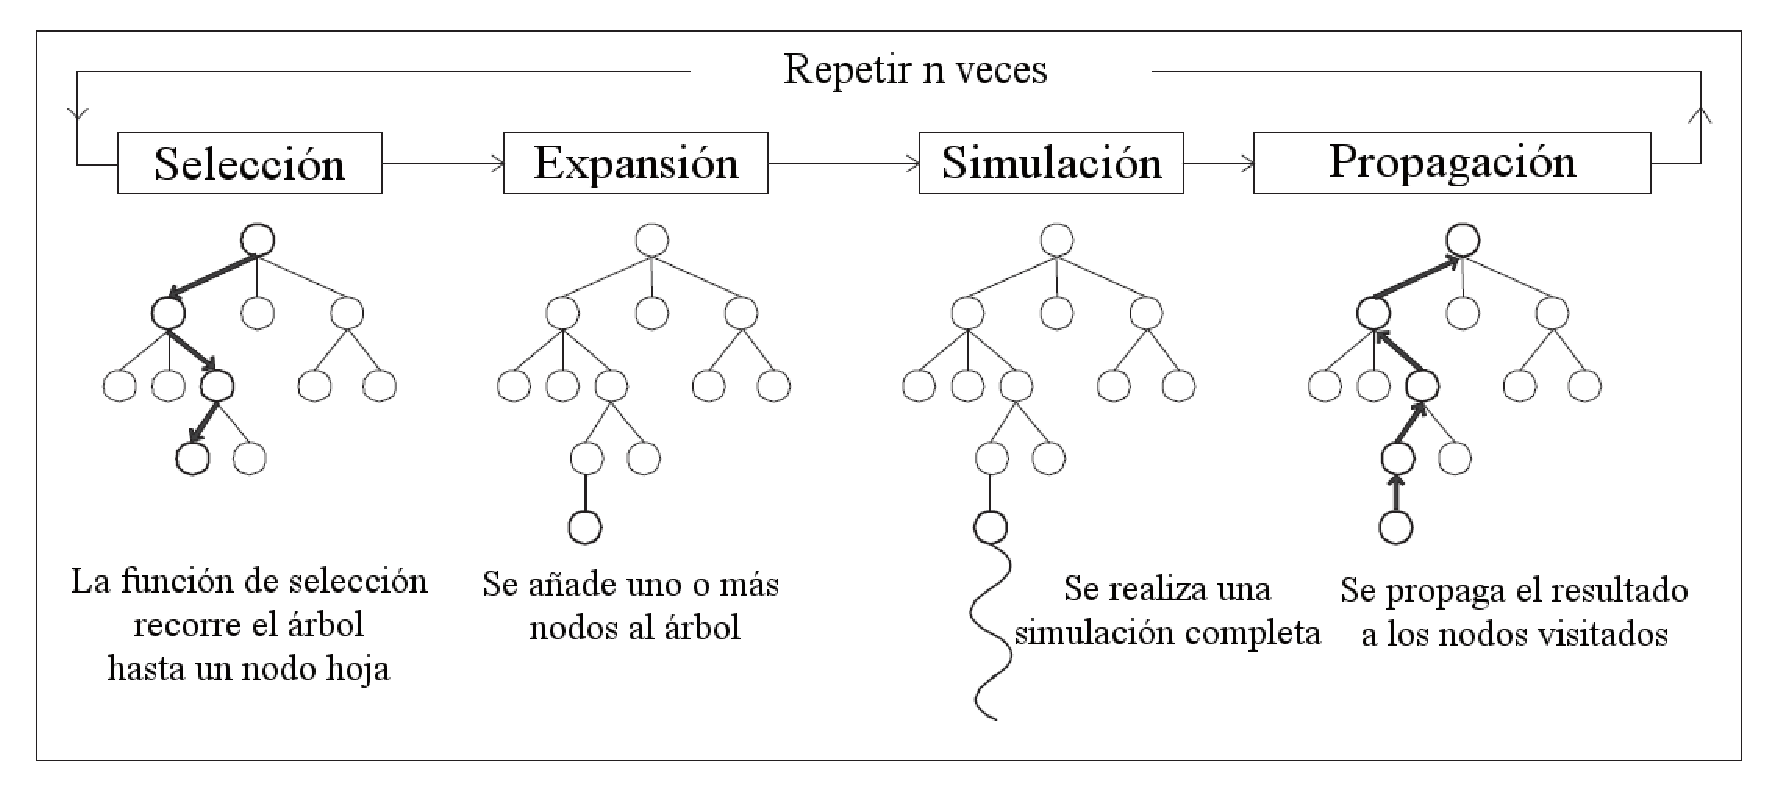
\includegraphics[scale=0.45]{contenido/cap3/imagenes/mcts1.eps}
	\caption[Fases del algoritmo Monte-Carlo Tree Search.]%
	{Fases del algoritmo Monte-Carlo Tree Search. (Imagen adaptada de \citeref{MCTS}.)}
	\label{fig:mcts1}
\end{figure}
La figura~\ref{fig:mcts1} muestra este proceso, que se puede dividir en cuatro fases:
selección, expansión, simulación y propagación.
Antes de detallar cada una de estas fases conviene definir la información que almacenará el árbol MC en cada nodo.

Sea \textit{s} el estado actual, el nodo correspondiente en el árbol MC contiene tres valores:
\begin{itemize}
	\item Número total de simulaciones realizadas desde el estado \textit{s}, que denotamos como \textit{N(s)}.
	\item Número total de simulaciones en las que se selecciona el movimiento \textit{a} desde el estado \textit{s}, que llamamos \textit{N(s,a)}.
	\item El valor Monte-Carlo del estado (valor MC), representado por \textit{Q(s,a)}, es el resultado promedio de todas las simulaciones realizadas en las que se seleccionó el movimiento \textit{a} en el estado \textit{s}:
	\begin{displaymath}
	Q(s,a)=\frac{1}{N(s,a)}\sum_{i=1}^{N(s)}\mathds{I}_i(s,a)z_i
	\end{displaymath}
	donde $z_i$ es el valor de utilidad devuelto por la \textit{i}-ésima simulación, y $\mathds{I}_i(s,a)$ es un indicador que vale 1 si el movimiento \textit{a} fue seleccionado en el estado \textit{s} durante la simulación \textit{i} y 0 en otro caso.
	Nótese que $N(s,a) = \sum_{i=1}^{N(s)}\mathds{I}_i(s,a)$.
\end{itemize}

La información almacenada puede variar dependiendo de la estrategia de selección que se use en la primera fase, aunque aquí se ha usado la información genérica que se puede obtener mediante las simulaciones, es decir, sin emplear conocimiento experto sobre el entorno.

A continuación se detalla cada una de las fases del algoritmo MCTS:
\begin{enumerate}
	\item \textbf{Selección} \\
	Partiendo del estado actual, se realiza una búsqueda en el árbol de juegos hasta encontrar un nodo que no está en el árbol MC.
	Los movimientos realizados en esta búsqueda están elegidos acorde a la información almacenada en el propio árbol MC, siguiendo una determinada estrategia.
	
La estrategia elegida debe mantener un equilibrio entre explotación y exploración.
Se puede seleccionar en cada paso el mejor movimiento, lo que favorecerá la explotación; pero por otro lado, los movimientos menos prometedores todavía tienen que ser explorados a mayor profundidad, debido a la incertidumbre de la evaluación, lo que favorecería la exploración.

En función de la estrategia escogida, obtendremos diferentes versiones del algoritmo MCTS.
Al final de la sección se citan algunas extensiones de MCTS.

Usaremos una estrategia conocida como \textit{optimism in the face of uncertainty}\footnote{Puede traducirse como \textit{optimismo frente a la incertidumbre}.}, que favorece los movimientos con un valor más alto pero permite a su vez explorar aquellas acciones que todavía no han sido suficientemente exploradas.
Para ello, definimos $Q^\oplus(s,a)$ como el valor del movimiento \textit{a} desde el estado actual \textit{s} (valor MC) con una bonificación adicional que será más alta para los movimientos menos visitados:
\begin{displaymath}
Q^\oplus(s,a) = Q(s,a) + c\sqrt{\dfrac{\log N(s)}{N(s,a)}}
\end{displaymath}
donde \textit{c} es una constante de exploración con valores reales en el intervalo [0,1] y \textit{log} es el logaritmo natural (base \textit{e}).

El movimiento elegido, que llamamos $a^\ast$, será aquel que maximize el valor $Q^\oplus(s,a)$:
\begin{displaymath}
a^\ast = \max_a{Q^\oplus(s,a)}
\end{displaymath}

	\item \textbf{Expansión} \\
	Cuando se encuentra un estado que no aparece en el árbol MC, este se añade como un nuevo nodo.
	De esta forma el árbol se expande un nodo en cada simulación.

Una variante puede ser añadir al árbol MC cada estado que se visite en la búsqueda, aunque en la práctica, para reducir los requisitos de memoria, no se añaden todos los nodos en cada simulación.
Normalmente, sólo se añade un nodo al árbol MC en cada simulación: el primer nodo encontrado que no esté presente en el árbol MC.
Si aún así la limitación de la memoria supone un problema, es posible realizar varias simulaciones antes de añadir un nuevo nodo al árbol MC; o incluso podar antiguos nodos del árbol MC a medida que la búsqueda progresa.

	\item \textbf{Simulación} \\
A partir del nuevo estado almacenado en el árbol MC se realiza una simulación completa de la partida siguiendo la estrategia por defecto, esto es, realizando movimientos aleatorios hasta el final del juego.
Después se asigna el valor de utilidad \textit{z} al estado terminal: +1 si es ganador para el jugador, -1 si es perdedor y 0 si es empate.

%En un juego no todos los posibles movimientos tienen la misma probabilidad de jugarse
Obviamente, también puede emplearse en esta fase otra estrategia distinta para elegir los posibles movimientos, como una función heurística que asigne valores más altos a aquellos movimientos que tienen más probabilidad de ser jugados o que parecen más prometedores; pero esta mejora se sale de los objetivos del proyecto por lo que los agentes desarrollados usan la estrategia por defecto para esta fase.

	\item \textbf{Propagación} \\
	Una vez realizada la simulación, se actualiza la información de cada nodo en el árbol MC en función del valor de utilidad obtenido:
	\begin{displaymath}
		\begin{array}{l}
		N(s) \leftarrow N(s) + 1 \\
		N(s,a) \leftarrow N(s,a) + 1 \\ 
		Q(s,a) \leftarrow Q(s,a) + \dfrac{z - Q(s,a)}{N(s,a)} \\
		\end{array}
	\end{displaymath}

\end{enumerate}

El movimiento final seleccionado por MCTS en el estado actual será el movimiento mejor valorado en el árbol MC, es decir, el movimiento \textit{a} con un valor MC mayor.

La figura~\ref{fig:mcts2} muestra cinco simulaciones de MCTS en las que se va construyendo el árbol MC.
Se trata de una versión simplificada del algoritmo. 
Siguiendo con la misma terminología usada en minimax, los nodos de color negro corresponden a nodos \textit{MAX}, los blancos a \textit{MIN}.
Cada simulación obtiene un valor de utilidad (en el caso de la figura~\ref{fig:mcts2} el valor es 1 si gana \textit{MAX} y 0 si gana \textit{MIN}).
En cada simulación se añade un nuevo nodo al árbol y se actualiza el valor de cada nodo en el árbol con el valor de utilidad; también se actualiza el número de veces que se ha seleccionado cada nodo.
\begin{figure}[h]
	\centering
	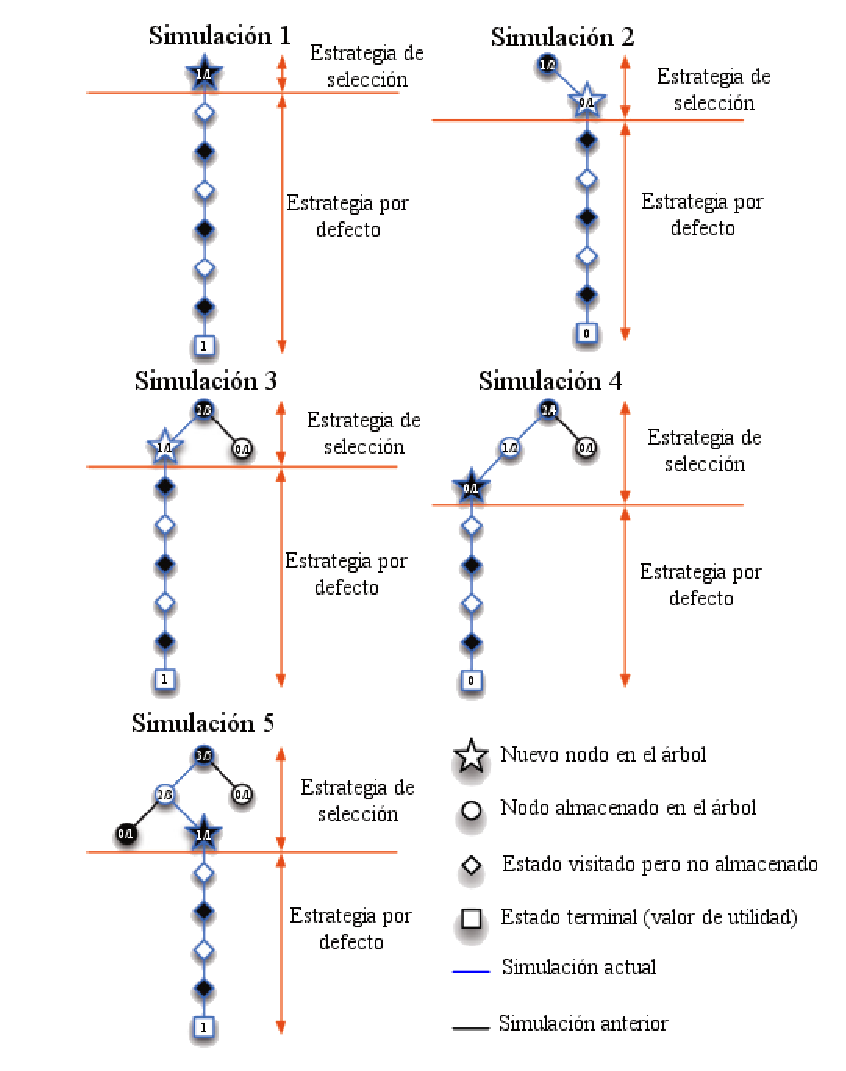
\includegraphics[scale=1]{contenido/cap3/imagenes/mcts2.eps}
	\caption[Cinco simulaciones de Monte-Carlo Tree Search.]%
	{Cinco simulaciones de Monte-Carlo Tree Search. (Imagen adaptada de \citeref{MCTS2}.)}
	\label{fig:mcts2}
\end{figure}
A medida que el árbol MC crece con cada simulación, los valores de los nodos se aproximan al valor minimax real y por tanto la estrategia basada en las simulaciones también se aproxima a la estrategia óptima de minimax.

\clearpage	% le dice a Latex que suelte todas las figuras en una página y comience una página nueva (detallado en los apuntes de los indios).

\bigskip
A continuación se presentan brevemente cuatro extensiones de MCTS en función de la estrategia elegida en las fases de selección y simulación.

\subsubsection{Extensiones de Monte-Carlo Tree Search}
\label{sssec:extensiones_MCTS}
El rendimiento de MCTS puede mejorarse significativamente si se incorpora información del dominio a la estrategia usada en la fase de selección o incluso a la estrategia por defecto usada en la fase de simulación.
Existen varias extensiones de MCTS basadas en la estrategia elegida para ambas fases, algunas extensiones son:
\begin{itemize}
	\item \textbf{\textit{Greedy MCTS}} \\
	La versión más básica de MCTS usa una estrategia \textit{best-first} (primero el mejor) que favorece la explotación frente a la exploración en la fase de selección.
A este algoritmo se le conoce como \textit{greedy MCTS}.
	\item \textbf{Algoritmo \textit{UCT}} \\
	El algoritmo \textit{UCT} (\textit{Upper Confidence bounds applied to Trees}, traducido como \textit{límites superiores de confianza aplicados a los árboles}). 
Usa el principio \textit{optimism in the face of uncertainty} que puede usarse para explorar el árbol de forma eficiente, ya que favorece a los movimientos con mayor valor potencial.
	Nuestra versión MCTS desarrollada se basa en este algoritmo.
	\item \textbf{\textit{Heuristic MCTS}} \\
	Utiliza funciones heurísticas con información del dominio para inicializar los valores de las nuevas posiciones en el árbol MC.
	\item \textbf{\textit{MC-RAVE}} \\
	Utiliza el algoritmo \textit{RAVE} (\textit{Rapid Action Value Estimation}), que mejora el método original compartiendo los valores de diferentes subárboles del árbol MC, por ejemplo en el caso de las transposiciones.
\end{itemize}
\citeref{MCTS2} contiene información detallada sobre estas extensiones de MCTS.

\bigskip
Explicada la estrategia MCTS, se presentan a continuación los agentes que la usan; al igual que ocurrió con el método básico de Monte-Carlo se trata de dos agentes: uno con un número de simulaciones fijado de antemano y otro con un límite de tiempo.

\subsubsection{Monte-Carlo Tree Search con número de simulaciones fijas}
\label{sssec:montecarloTreeSearch_simulaciones}
El primer agente que usa MCTS realiza un número de simulaciones determinado.

Partiendo del estado actual, ejecuta el ciclo de cuatro fases presentado anteriormente tantas veces como indique el número de simulaciones asignado.
Establecer el número de simulaciones en MCTS es aún más difícil que para el agente Monte-Carlo básico porque ahora cada simulación necesita más tiempo para llevarse a cabo debido a que debe gestionar el árbol MC.

Por otro lado, el agente dispone de una opción que permite reutilizar el árbol MC de un movimiento para el siguiente, ya que los valores del árbol son válidos de un movimiento a otro.
Esto permite mejorar la evaluación de los movimientos a medida que el agente juega la partida, a costa de incrementar los recursos necesarios (en memoria y tiempo) para manejar el árbol MC.
Recordemos que el árbol se expande un nodo en cada simulación.

Este agente tiene también un parámetro perteneciente a la constante de exploración \textit{c} que se vio en la fase de selección.
El parámetro permite ajustar la estrategia de selección favoreciendo la exploración (valores próximos a 1) o la explotación (valores próximos a 0).

El último agente también usa MCTS para evaluar el mejor movimiento, pero esta vez dispone de un tiempo limitado para devolver el movimiento.

\subsubsection{Monte-Carlo Tree Search con límite de tiempo}
\label{sssec:montecarloTreeSearch_limiteTiempo}
Este agente usa MCTS con un límite de tiempo para realizar las simulaciones, esto es, las iteraciones completas de cuatro fases de MCTS (selección, expansión, simulación y propagación).

Las iteraciones deben completarse totalmente para que sean válidas; de ahí que asignar el límite de tiempo no sea una tarea trivial.
Si cada iteración necesita más tiempo del disponible, el tiempo límite del agente se extenderá hasta completar la última iteración.
El límite de tiempo viene expresado en segundos al igual que el resto de jugadores con límite de tiempo que se han desarrollado.

Este agente también cuenta con la opción de reutilizar el árbol MC de un movimiento a otro; y también tiene parámetro para ajustar el nivel de exploración en la fase de selección.
